% Template for ICASSP-2010 paper; to be used with:
%          mlspconf.sty  - ICASSP/ICIP LaTeX style file adapted for MLSP, and
%          IEEEbib.bst - IEEE bibliography style file.
% --------------------------------------------------------------------------
\documentclass{article}
\usepackage{amsmath,graphicx, mlspconf}

%***CHEMISTRY PACKAGES***%
\usepackage[version=4]{mhchem}

% *** CITATION PACKAGES ***
%
\usepackage{cite}

%% *** SUBFIGURE PACKAGES ***
%\usepackage[caption=false,font=normalsize,labelfont=sf,textfont=sf]{subfig}
\usepackage[caption=false,font=footnotesize]{subfig}

\usepackage{lipsum}

\usepackage{fixltx2e}

\usepackage{multirow,siunitx}

\toappear{2019 IEEE International Workshop on Machine Learning for Signal Processing, Oct.\ 13--16, 2019, Pittsburgh, PA, USA}

% Example definitions.
% --------------------
\def\x{{\mathbf x}}
\def\L{{\cal L}}

% Title.
% ------
\title{Non-audible Speech Recognition from EMG signals using Deep Learning}
%
% ---------------
\name{Rommel Fernandes, Lei Huang, Gustavo Vejarano}
\address{Loyola Marymount University\\
         Department of Electrical Engineering and Computer Science\\
         Los Angeles, CA, USA\\
         rferna16@lion.lmu.edu, lei.huang@lmu.edu, gustavo.vejarano@lmu.edu}
%
% For example:
% ------------
%\address{School\\
%	Department\\
%	Address}
%
% Two addresses (uncomment and modify for two-address case).
% ----------------------------------------------------------
%\twoauthors{A. Author-one, B. Author-two.}}
%\address{School A-B\\
%	     Department A-B\\
%	     Address A-B}
%   Email A-B
%  {C. Author-three, D. Author-four\sthanks{The fourth author performed the work
%	while at ...}}
%	{School C-D\\
%	Department C-D\\
%	Address C-D
%   Email C-D}
%
\begin{document}
%\ninept
%
\maketitle
%
\begin{abstract}
Research advancement of Human-Computer Interaction has recently been made to help post-stroke victims dealing with physiological problems such as speech impediments due to aphasia. This paper investigates different deep learning models used for non-audible speech recognition from Electromyography (EMG) signals. A novel approach employing Continuous Wavelet Transforms (CWT) and Convolutional Neural Networks (CNNs) were proposed to recognize silent speeches. To compare its performance with other popular deep learning approaches, we collected facial surface EMG bio-signals from subjects with binary and multi-class labels, trained and tested four different deep learning models, including a Long-Short Term Memory(LSTM) model, a bi-directional LSTM model, a 1-D CNN model, and our proposed CWT-CNN model.  Experimental results showed that our proposed approach performs better than the LSTM models, but is less efficient than the 1-D CNN model on our collected data set. In comparison with previous research,  we gained insights on how to improve the performance of the model for binary and multi-class silent speech recognition. 
\end{abstract}
%
\begin{keywords}
Deep Learning, Electromyography, Silent Speech Interfaces, Human-Computer Interaction
\end{keywords}
%
\section{INTRODUCTION}
\label{sec:INTRODUCTION}

Over the past few years, HCI has been an increasing field of study. HCI can be described as a feedback loop between human and computer. With the increased usage of wearable devices, such as watches, heart rate monitors, and other smart sensors, researchers extract bio-signal information to recognize typical human activities.  For example, electrocardiogram (ECG) signals have been used to detect irregular heartbeats ~\cite{noauthor_classify_nodate}, while electroencephalography (EEG) ~\cite{eltvik_deep_nodate} and electromyography (EMG)  ~\cite{altamirano_emg_nodate} signals have been used to predict body movements. 

Silent Speech Interface(SSI) is one type of HCI, aiming at It employs signal-extracting systems, such as EMG and/or EEG, to collect signals of silent or non-audible speech, then recognizing different meanings represented by the signals using machine learning algorithms. SSI systems can help post-stroke victims dealing with physiological problems such as speech impediments due to aphasia. In the past, machine learning algorithms typically used for speech recognition, such as decision tree, support vector machine, Naïve Bayes, and Hidden Markov Models, were also employed as classifiers for silent speech signals. These traditional machine learning algorithms require extensive feature extraction from signals, and only shallow features can be learned from those approaches, leading to undermined performance. ,With recent advancement in deep learning and its breakthrough performance applied to speech recognition, state-of-the-art SSI systems have employed deep learning  technologies to classify silent speech signals. ~\cite{wang_deep_2017}.

This paper focuses on recognizing EMG captured non-audible speech, which is caused by the inability to verbalize words or sentences through the use of sound in an effective way. Compared with other methods to capture non-audible speech such as Electroencephalography (EEG), Near infrared sensors (fNIRS), implants for speech and motor cortex (ECOG), and video camera lip reading, EMG is non-invasive and most cost-effective. Therefore, we employ EMG to capture non-audible speech in our project. Then, we investigate different deep learning models, including both Recurrent Neural Networks (RNNs) and Convolutional Neural Networks (CNNs) as the classifier for recognizing the captured EMG signals. In general, RNN models such as LSTM are prevalent in modeling time-sequence signals including speech, while CNN models are used for multidimensional signals such as images and videos. Similar to speech signals, EMG signals are time sequences, which are suitable for RNN modeling. On the other hand, EMG signals are always collected through multiple sensor arrays  placed at different locations, it can also be arranged as multidimensional tensors, which are suitable for CNN modeling.  In this work, we compare RNN and CNN models for classifying EMG signals. In addition, we propose a novel approach to applying CNN on the scalograms of EMG signals through a continuous wavelet transform,  

The rest of this paper is organized as follows. Section \ref{sec:RELATED WORK} discusses several recent works related to our work. Section \ref{sec:SYSTEM DESCRIPTION} describes our experimental setup used to capture, analyze, and model the data. Section \ref{sec:EXPERIMENTAL MODELS}  discusses the specific models being used in our proposed solution. Section \ref{sec:PROPOSED SOLUTION}  presents our proposed solutions. Section \ref{sec:EXPERIMENTAL RESULTS} discusses the results from our analysis and compares them to the related work. Finally, Section \ref{sec:CONCLUSION} concludes this paper with recommendations for future work.

\section{RELATED WORK}
\label{sec:RELATED WORK}

Research conducted using EMG to predict speech for SSI systems has been undergone for over two decades. Before the deep learning era, using EMG to recognize speech patterns involved heavy feature extraction of the data, along with discrete mathematical modeling. Recently, there have been well documented results that have used a combination of mathematical modeling and deep learning to predict speech using EMG. Some research addresses syllable and single word based prediction ~\cite{lopez-larraz_syllable-based_2010}, ~\cite{maier-hein_session_2005}. Other research has addressed using EMG to predict entire phrases ~\cite{janke_emg--speech:_2017}, ~\cite{kapur_alterego:_2018}.

One of the earliest attempts to use EMG to predict speech was done in ~\cite{maier-hein_session_2005}. The goal was to predict isolated words from a vocabulary consisting of the ten English digits \textit{0-9}. Seven electrodes were positioned on the face to extract bio-signals from the subjects. Hidden Markov Models (HMM) with Gaussian Mapping Models (GMM) were used as classifiers. 

In ~\cite{wand_pattern_2014}, new approaches with machine learning models were introduced, such as Restricted Boltzmann Machine algorithms and Deep Neural Networks (DNN). Their corpus consisted of 25 sessions from 20 speakers comprising of 200 read English-language utterances such as phonemes, consonants, and vowels. Their results showed that DNN models performed better for phoneme related classifications using EMG inputs. 

The work performed by ~\cite{janke_emg--speech:_2017} continued some of the primary research done by ~\cite{wand_pattern_2014}. This research investigated bidirectional LSTMs, and compared it with other models such as GMMs. Their results showed that LSTM models performed better than that of GMM.

The work done by ~\cite{diener_session-independent_nodate} used the same data set and corpus of ~\cite{janke_emg--speech:_2017}. Their primary work focused on evaluating the performance of CNN based models for EMG-to-Speech conversion. The researchers converted EMG signals to mel-frequency cepstral coefficients (MFCCs) and extracted feature vectors from multiple channels, and then used two CNN based models,  a LeNet-inspired model, and a ResNet-32 based encoder-decoder model, to  Their results showed that the CNN based architectures are able to outperform a plain DNN based conversion system.

In ~\cite{kapur_alterego:_2018}, the authors built a proof of concept SSI system that used a one-dimensional CNN as a classifier. Seven electrodes were placed around the throat and face.  Subjects in the research do not open their mouth, make any sound, or provide any muscle articulation in order to train the models. Their quantitative results for the one-dimensional CNN network reported an average accuracy of 92.01\% for all subjects. Their corpus included individual words and short phrases.

From the above mentioned research work, it has been shown that deep learning models have improved the performance of EMG signal modeling over traditional models, and CNN models outperform plain DNN models. However, there has not been any comparison between RNN and CNN in recognizing EMG silent speech signals. In addition, some previous research  applied models on extracted feature vectors of EMG signals, while others on the original data collected. Inspired by these observations, we compare the performance of several RNN and CNN models, and propose a different data representation method using wavelet transformed signals, which provides time-frequency information of the signals.  

\section{SYSTEM DESCRIPTION}
\label{sec:SYSTEM DESCRIPTION}

The system we used in our experiments consists of three main subsystems. In the data acquisition, original multi-channel  EMG data are collected from 10 different human subjects who volunteered to participate in the experiment. The collected raw data are then cleaned, aligned and labeled with corresponding labels in the data preprocessing stage. Then appropriately formatted and divided data sets are used to train and test different deep learning models that recognize the EMG signals. In the following subsections, we describe each subsystem in detail. 

\subsection{Data Acquisition}
\label{ssec:Capturing Data}
Since our main focus is on comparing different deep learning models, we simplified our data acquisition process by using three channels positioned on the cheek and throat area as suggested in ~\cite{maier-hein_session_2005}. Compared to far greater number of channels used in previous work in\cite{kapur_alterego:_2018}, ~\cite{wand_pattern_2014}, ~\cite{janke_emg--speech:_2017}, ~\cite{maier-hein_session_2005}, this minimum number of electrodes reduced discomfort experienced by human subjects participated in the experiment. 

The data acquisition device consists of two Shimmer3 EMG units, each with a 24 MHz CPU. The EMG units have the capability of recording two channels of data using \ce{Ag/AgCl} bipolar electrodes with a reference electrode connected to a bone-dense area. The bipolar electrodes are placed strategically based on work done in ~\cite{lopez-larraz_syllable-based_2010}. The areas where the EMG electrodes are placed are as follows. \textit{Depressor anguli oris} (EMG1), \textit{Zygomaticus major} (EMG2), and \textit{Anterior belly of the digastric} (EMG3). Each bipolar electrode of the muscle group is placed approximately 2 cm apart based on the unit specifications in (\figurename \ref{Fig. 1b}). After proper placement of the electrodes on a subject, the EMG units are placed on the subjects upper torso and shoulder, using comfort straps.  Data including the EMG signal strength and timestamps is transmitted via Bluetooth to a Linux (Ubuntu) Intel laptop using  open source Python programs. Details about data capture and cleaning up are described in the following subsections. 

After the subject is connected to the EMG units with the electrodes in place, the process of acquiring EMG data with annotated samples begins. In our experiments, we are capturing two types of labeled annotations for our sample data. Our \textit{first set} of annotations consists of the labels for the words \textit{yes} and \textit{no}. Our \textit{second set} of annotations consists of the labels of the numeric digits \textit{0-9}. The annotations are generated at random using a python script that prints out the label for the subject to read  (\figurename \ref{Fig. 1a}). The label persists on the screen for two seconds; it is then followed by the word \textit{relax}, which persists on the screen for two more seconds. The next label in the annotations is displayed and repeated at random for a total of 50 labels per annotated set. The subject performs this task for the \textit{first set} and \textit{second set}. The associated EMG signals captured with the annotated labels will be used to train the various deep learning models, which will be discussed in Section \ref{ssec:Experimental models}.  

\begin{figure}[!b] 
    \centering
  \subfloat[Annotated labels displayed on screen for subject to read\label{Fig. 1a}]{%
       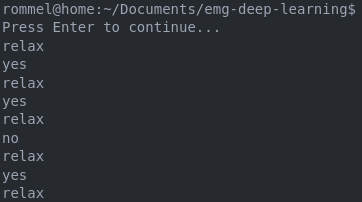
\includegraphics[width=0.65\linewidth]{images/annotations.png}}
    \\
  \subfloat[Connections to speech-focused muscle groups for EMG data.\label{Fig. 1b}]{%
        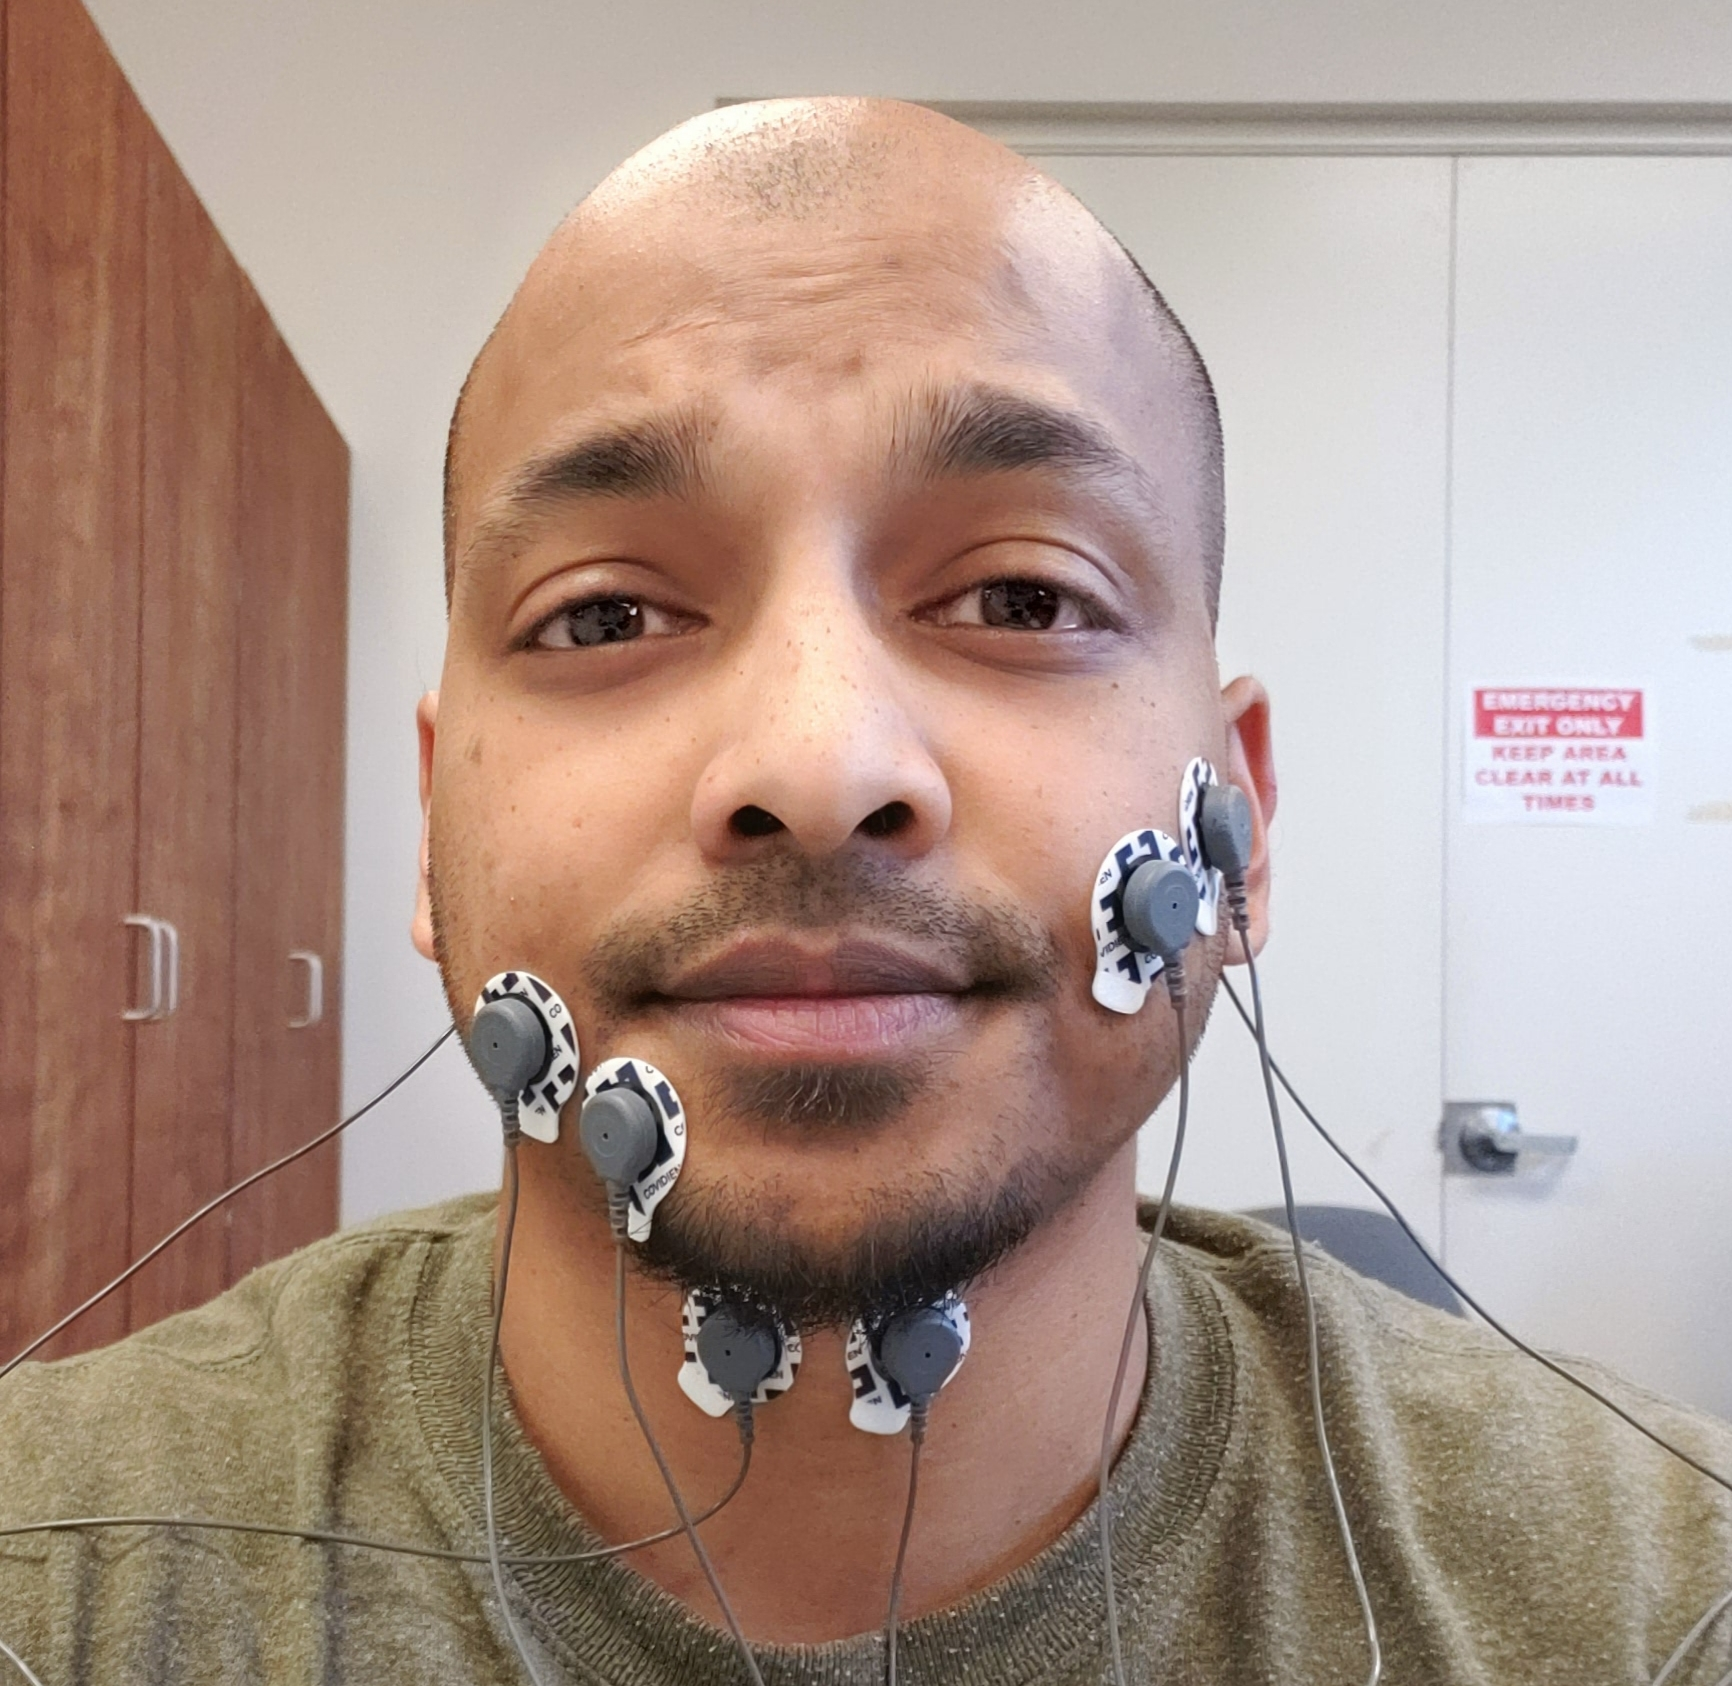
\includegraphics[width=0.65\linewidth]{images/face_leads.jpg}}
  \caption{Subjects reading annotated labels on screen while connected to EMG units and electrodes.}
  \label{fig: conn-ann} 
\end{figure}

%\section{TYPE-STYLE AND FONTS}
%\label{sec:typestyle}

\subsection{Data Preprocessing}
\label{ssec:Cleaning Data}
Once the data is captured from the subjects, it has to be cleaned and aligned before being input to deep learning models. In order to remove the noises from the signals, both low-pass and high-pass filters are applied. We also want to eliminate the 60 Hz interference from the surroundings. First, we applied a low-pass filter with a cutoff frequency of 4 Hz, assuming  muscle movements are mostly below 4 Hz. Then, we applied a high-pass filter with a cutoff frequency of 0.5 Hz, which removes the associated DC offset. The filters are designed around a window sinc function ~\cite{noauthor_how_nodate}. The coinciding timestamps of the EMG data with the annotations are mapped together to create an input-output relationship. \figurename \ref{fig: cleaned_signals} shows some samples of the preprocessed EMG signals from three channels with the respective annotated labels, which will be  used for training and testing of the models. 

\begin{figure}[!t]
\centering
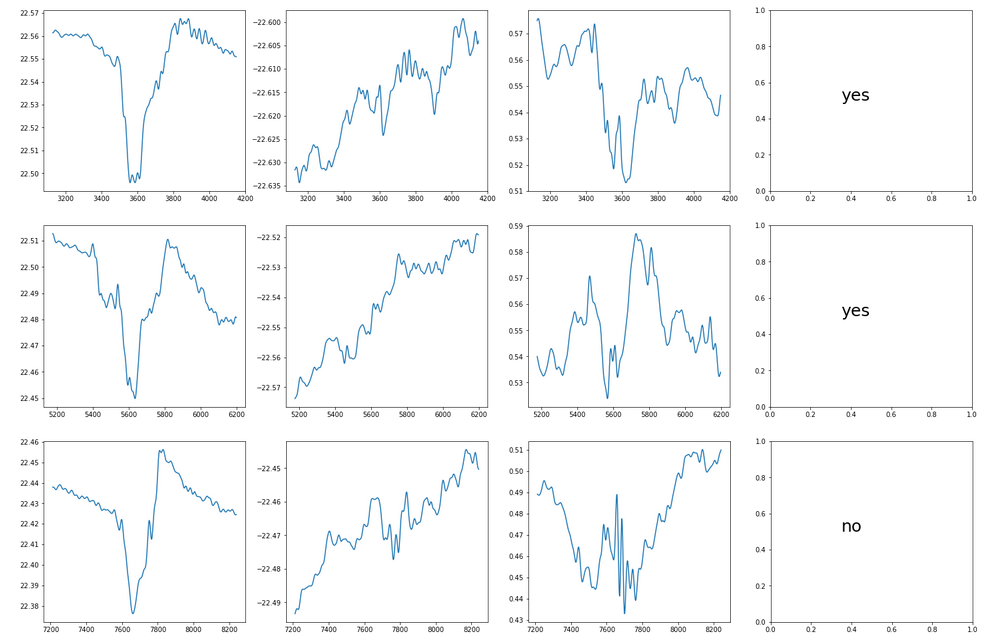
\includegraphics[width=3.5in]{images/cleaned_signals.png}
\caption{Signals after cleaning and adding low-pass and high-pass filters. First Column: EMG1, Second Column: EMG2, Third Column: EMG3, Fourth Column: Annotated Labels}
\label{fig: cleaned_signals}
\end{figure}

\subsection{Model Training and Testing}
\label{ssec:Experimental models}
The preprocessed data sets are divided into training/testing subsets by a 80/20 split. We 
\textit{Recurrent neural networks} (RNN), in particular LSTMs, are an effective tool for sequence processing that learn hidden representations of their sequential input. An LSTM can use its memory cells to remember long-range information and keep track of various attributes of data it is currently processing ~\cite{karpathy_visualizing_2016}. An LSTM is built from an RNN, which works by unrolling data into N different copies of itself. Input of data from previous time steps $t_{n-1}$, $t_{n-2}$, $t_{n-3}$ \ldots, $t_{0}$ can be used when the current time-step $t_{n}$ is being evaluated. RNNs can learn temporal dependencies in the sequential data, and use it to classify new data. These unique capabilities make RNNs and LSTMs ideal for classification of time-series data such as EMG signals. Adding multiple layers to LSTMs can improve results of speech recognition, as investigated by ~\cite{graves_speech_2013}. In our experiment, we will use the sequential data from each EMG channel to classify the annotated labels in our data sets.

Another deep learning model that we investigated are \textit{Convolutional Neural Networks}. CNN takes multi-resolutional local spatial information into consideration by applying a number of learnable filters in multiple layers.  CNN models are ideal for identifying spatial patterns from image data. 1-D CNN models have also been applied in time-series data such as language and EMG signal modeling.  In order to convert sequential time-series data into image representations, we investigated \textit{Continuous Wavelet Transforms}(CWT). Unlike Fourier transform approaches that only show a signal representation in the frequency domain, wavelet transforms show both time and frequency representations. In ~\cite{janke_emg--speech:_2017}, ~\cite{kapur_alterego:_2018}, ~\cite{diener_session-independent_nodate}, they generated mel-frequency cepstral coefficients (MFCC), which creates one-dimensional representation that closely characterizes the envelopes of human speech as features in their respective models. In ~\cite{huzaifah_comparison_2017}, however states that time-frequency representations such as the CWT produced better results in terms of accuracy than the MFCC features. The wavelet transform of a one-dimensional signal will generate coefficients as a two-dimension matrix of time-frequency representations, which is also known as a scaleogram. This scaleogram gives information about the dynamic behavior of the system, similar to that of a distinguishable image. Therefore, we propose a CWT based representation of EMG signals with 2-D CNN models  for the classification of EMG signals ~\cite{pauk_419._2008} by using CNN models ~\cite{huzaifah_comparison_2017}.

\section{PROPOSED SOLUTION}
\label{sec:PROPOSED SOLUTION}

Once the data is filtered and transformed, it will be ready for modeling. We used the two second window samples of when the subject repeated an annotated label on the screen and dropped the instances where the word \textit{relax} existed. In our first proposed solution, we experimented with an LSTM model. The model is single direction LSTM, similar to ~\cite{janke_emg--speech:_2017},that consists of a LSTM layer with 100 filters followed by a Dense layer of 80 filters, and an output layer. The LSTM model is comprised of commonly used hyper-parameter values, such as a batch size of 32, with a learning rate of \textit{1e-4}. To measure the loss of the model, we used binary cross-entropy for the binary cases of \textit{yes} and \textit{no}, and categorical cross-entropy for the cases \textit{0-9}. We followed a many to one, sequence input architecture for the LSTM. The many to one architecture allows us to map many input sequences, in our case three, to a single output.

For our second experiment, we used a CNN architecutre as a deep learning model. We converted our singals into wavelet transforms, which generated scalograms that show resolution in the frequency and time-domains ~\cite{wletCNN}. Since there are three EMG channels of data, we created three sclaeograms per label, \figurename \ref{fig: wavelet_signals}. We then placed the three scaleograms on top of each other and created an image representation. The coefficients from the output of the scaleogram is then utilized as features to train the CNN model. The CNN architecture, similar to Lenet, is a two-layer model with a structure that can be represented as conv1-pool1-conv2-pool2-flat-dense-FC, with a  0.5 dropout before FC layer. The hidden convolutional layers have a size of 32, 64, and 512 filters respectively. The convolutional layers have a filter size of 3x3, and a max-pooling kernel size of 2x2, with a stride of 2. The hyper-parameters include a learning rate of \textit{1e-4} and batch size of 16. A smaller batch size is due to the fact of the large tensor size of the training data. Finally for the CWT parameters, we choose frequency bin size of 256 and a Mexican hat wavelet function. All of the models were trained on a Google Cloud Compute Engine with four virtual CPUs, 26 GB memory, and one NVIDIA Tesla K80 Graphics Processing Unit (GPU).

\begin{figure}[!tb]
\centering
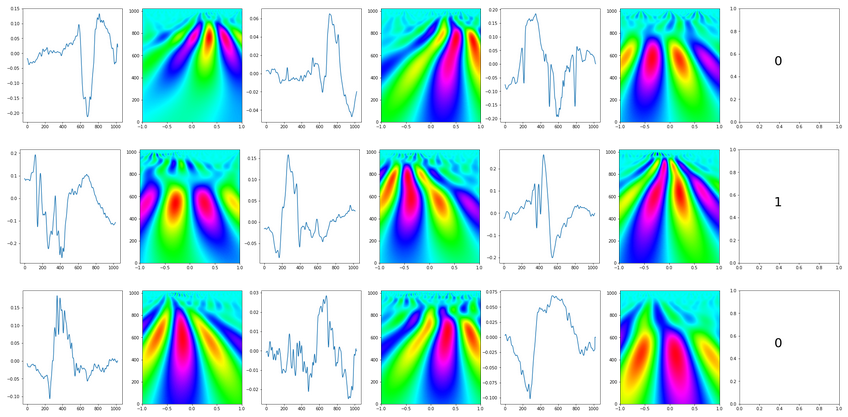
\includegraphics[width=3.5in]{images/wavelet_signal.png}
\caption{Continuous wavelet transform for each EMG channel as inputs, which maps to the labeled output.}
\label{fig: wavelet_signals}
\end{figure}

\section{EXPERIMENTAL RESULTS}
\label{sec:EXPERIMENTAL RESULTS}
To evaluate the performance of the deep learning models, we use precision and recall for each label, as well as the overall average precision and recall values. In short, recall measures the model's capability of identifying relevant samples over all relevant samples in the data set, while precision measures the fraction of correctly identified relevant samples over all identified relevant samples. 

\sisetup{table-format=2.2} 
\begin{table}[!h]
\centering
\caption{LSTM Model Results}
\begin{tabular}{|c|l|S|S|S|S|}           \hline 
\multirow{2}{*}{\# of class} &\multirow{2}{*}{label}    & \multicolumn{2}{c|}{Training Data}    &\multicolumn{2}{c|}{Testing Data}                    \\   \cline{3-6}
 &  &{Prec.} & {Rec.} & {Prec.}  & {Rec.}              \\   \hline 
\multirow{2}{*}{2} & no & 0.62 & 0.82 & 0.60  & 0.83   \\   \cline{2-6}  
 & yes & 0.72 & 0.47 & 0.77   & 0.52                \\   \hline
 \multicolumn{2}{|c|}{Average}   & 0.67 & 0.65 & 0.69 & 0.66 \\ \hline 
 \end{tabular}     
 %\caption{An important table}\label{Table. 1a}
 \label{Table 1: LSTM} 
\end{table}
 
\sisetup{table-format=2.2} 
\begin{table}[!h]
\centering
\caption{CWT-CNN Model Results }
\begin{tabular}{|c|l|S|S|S|S|}           \hline 
\multirow{2}{*}{\# of class} &\multirow{2}{*}{label}    & \multicolumn{2}{c|}{Training Data}    &\multicolumn{2}{c|}{Testing Data}                    \\   \cline{3-6}
 &  &{Prec.} & {Rec.} & {Prec.}  & {Rec.}              \\   \hline 
\multirow{2}{*}{2} & no & 0.97 & 0.95 & 0.75  & 0.72   \\   \cline{2-6}  
 & yes & 0.95 & 0.97 & 0.76   & 0.79                \\   \hline
 \multicolumn{2}{|c|}{Average}   & 0.96 & 0.96 & 0.76 & 0.76 \\ \hline 
 \end{tabular}     
 %\caption{An important table}\label{Table. 1a}
 \label{Table 2: CWT-CNN} 
\end{table}

Table \ref{Table 1: LSTM} shows the precision and recall for the LSTM model in our binary classification case. Table \ref{Table 2: CWT-CNN} shows the continuous wavelet transform with the CNN approach. The CWT-CNN model performs significantly better for both training and testing data sets when compared to the LSTM model. On average for the binary test cases of \textit{yes} and \textit{no}, the CWT-CNN model had precision score of 82\%, and the LSTM model had a precision score of 61.5\%. For the multi-class test cases of \textit{0-9}, the results were not as favorable with an average precision score around 10\% for both LSTM and CWT-CNN models.

\section{DISCUSSION}
\label{sec:DISCUSSION}

In comparison with  ~\cite{janke_emg--speech:_2017}, ~\cite{kapur_alterego:_2018}, ~\cite{diener_session-independent_nodate}, who used similar deep learning models, thier results achieved better accuracy when compared to the work in this paper. A  contributing factor to their increase in performance is the amount of data they had available for thier training and testing purposes. In ~\cite{kapur_alterego:_2018}, approximately 31 hours of training data was captured in order to train their one-dimensional CNN model. In ~\cite{janke_emg--speech:_2017}, ~\cite{diener_session-independent_nodate}, who trained a variety of different models, utilized on-going corpus of data from previous research projects that focused on EMG-SSI systems. We have shown for a small data corpus, CNN based models perform better than LSTM models. With additional data, we believe that our models for binary and multi-class labels can be on par with other EMG-SSI systems using deep learning that were researched in this paper.

One of the ways our model differentiates and possibly improves is the use of CWT over MFCC. The MFCC requires windowed sampling in small increments. The output of the MFCC are one-dimensional coefficients, while CWT outputs coefficients in two-dimensions, allowing deep learning models such as CNN to learn and extract more features ~\cite{huzaifah_comparison_2017}. In previous research, MFCC were primary used for shallow learning speech recognition models such as HMM. As deep learning and CNN models continue to gain popularity, the use of mult-dimensional transformation techniques such as CWT will become more prevalent for speech recognition SSI systems. 

The transformation of data, specifically one-dimensional signals to its time-frequency components requires significant processing power. Resource limited systems cannot perform such laborious processes. We trained our models on a cloud computing engine which had the capability of increasing CPU and GPU power. These systems can become costly as the number of dedicated resources are assigned to the task of training a model. One has to justify the efforts of performance versus cost, specifically if the models improvements are only a few percentage. In terms of speech recognition, accuracy is important, the ability recognize speech patterns from a SSI system with high accuracy is a long-term goal.  

% Below is an example of how to insert images. Delete the ``\vspace'' line,
% uncomment the preceding line ``\centerline...'' and replace ``imageX.ps''
% with a suitable PostScript file name.
 -------------------------------------------------------------------------

%\begin{figure}[htb]
%
%\begin{minipage}[b]{1.0\linewidth}
%  \centering
%  \centerline{\includegraphics[width=8.5cm]{image1}}
%%  \vspace{2.0cm}
%  \centerline{(a) Result 1}\medskip
%\end{minipage}
%%
%\begin{minipage}[b]{.48\linewidth}
%  \centering
%  \centerline{\includegraphics[width=4.0cm]{image3}}
%%  \vspace{1.5cm}
%  \centerline{(b) Results 3}\medskip
%\end{minipage}
%\hfill
%\begin{minipage}[b]{0.48\linewidth}
%  \centering
%  \centerline{\includegraphics[width=4.0cm]{image4}}
%%  \vspace{1.5cm}
%  \centerline{(c) Result 4}\medskip
%\end{minipage}
%%
%\caption{Example of placing a figure with experimental results.}
%\label{fig:res}
%%
%\end{figure}

% To start a new column (but not a new page) and help balance the last-page
% column length use \vfill\pagebreak.
% -------------------------------------------------------------------------
%\vfill
%\pagebreak

\section{FUTURE WORK}
\label{sec:FUTURE WORK}

One of the main ways to improve accuracy in our models is to acquire more training data. Getting subjects to volunteer can at times be challenging, more importantly annotating EMG data with proper labels. Acquiring more data would allow us to also train a variety of words and phrases, so that we can eventually build a robust SSI system. In our model, we eliminated instances where the subject was told to \textit{rest}. Future models should incorporate the \textit{rest} instances as an additional class, so that the model will learn to identify false positives.

The eventual goal is to build an SSI system that can improve its word recognition capablity over time as more data from similar SSI systems relay information over the network; resembling a Wireless Sensor Network and the Internet of Things ~\cite{ferdoush_wireless_2014}. A Bluetooth SSI system would communicate with a base station, process the data through the model, and output the results via an audio or visual interface. As more data is collected, deep learning models would be updated in the cloud, and pushed back to the base stations for processing.

\section{CONCLUSION}
\label{sec:CONCLUSION}

We have shown by using well-known deep learning methods we can effectively create models to recognize non-audible speech using surface EMG. This type of research is critical in designing SSI systems that can be used to interface with people who suffer from speech related problems. The experiments conducted by gathering data from a small sample of subjects showed that, CNN models tend to perform better than LSTM models, in terms of speed, accuracy, and precision in recognizing non-audible speech. Our approach of CWT with a combination of CNN also led to similar results when compared to previous research; however, the cost of running such model may outweigh the benefits. In the future, finding ways to capture more robust data will be critical in training precise models that can disseminate and recognize a variety of words or phrases for SSI systems.

% References should be produced using the bibtex program from suitable
% BiBTeX files (here: strings, refs, manuals). The IEEEbib.bst bibliography
% style file from IEEE produces unsorted bibliography list.
% -------------------------------------------------------------------------
\bibliographystyle{IEEEbib}
\bibliography{first_draft}

\end{document}
